\subsection{Теория информации}
	
	\subsubsection{Аннотация}

		Курс <<Теория информации>> получил смешанные отзывы. Основные проблемы -- это поверхностное прохождение программы. Возможно, стоит меньше заострять внимание на очевидные моменты в курсе, чтобы затронуть наибольшее количество тем в семестре.
		
		Руководствуясь результатами опроса, Совет студентов и аспирантов ФРКТ выдвигает следующие идеи по улучшению данного курса:
		\begin{enumerate}
			\item расширить программу курса, добавив больше тем и углубленных материалов;
			\item рассказывать о практических применениях теории в курсе;
			\item рассмотреть возможность переноса курса на более ранний семестр (1-2 курс), чтобы он был более актуальным и полезным для студентов.
		\end{enumerate}

	\subsubsection{Общий отзыв студентов о курсе}

		\begin{figure}[H]
			\centering
			\begin{subfigure}[b]{0.45\textwidth}
				\centering
				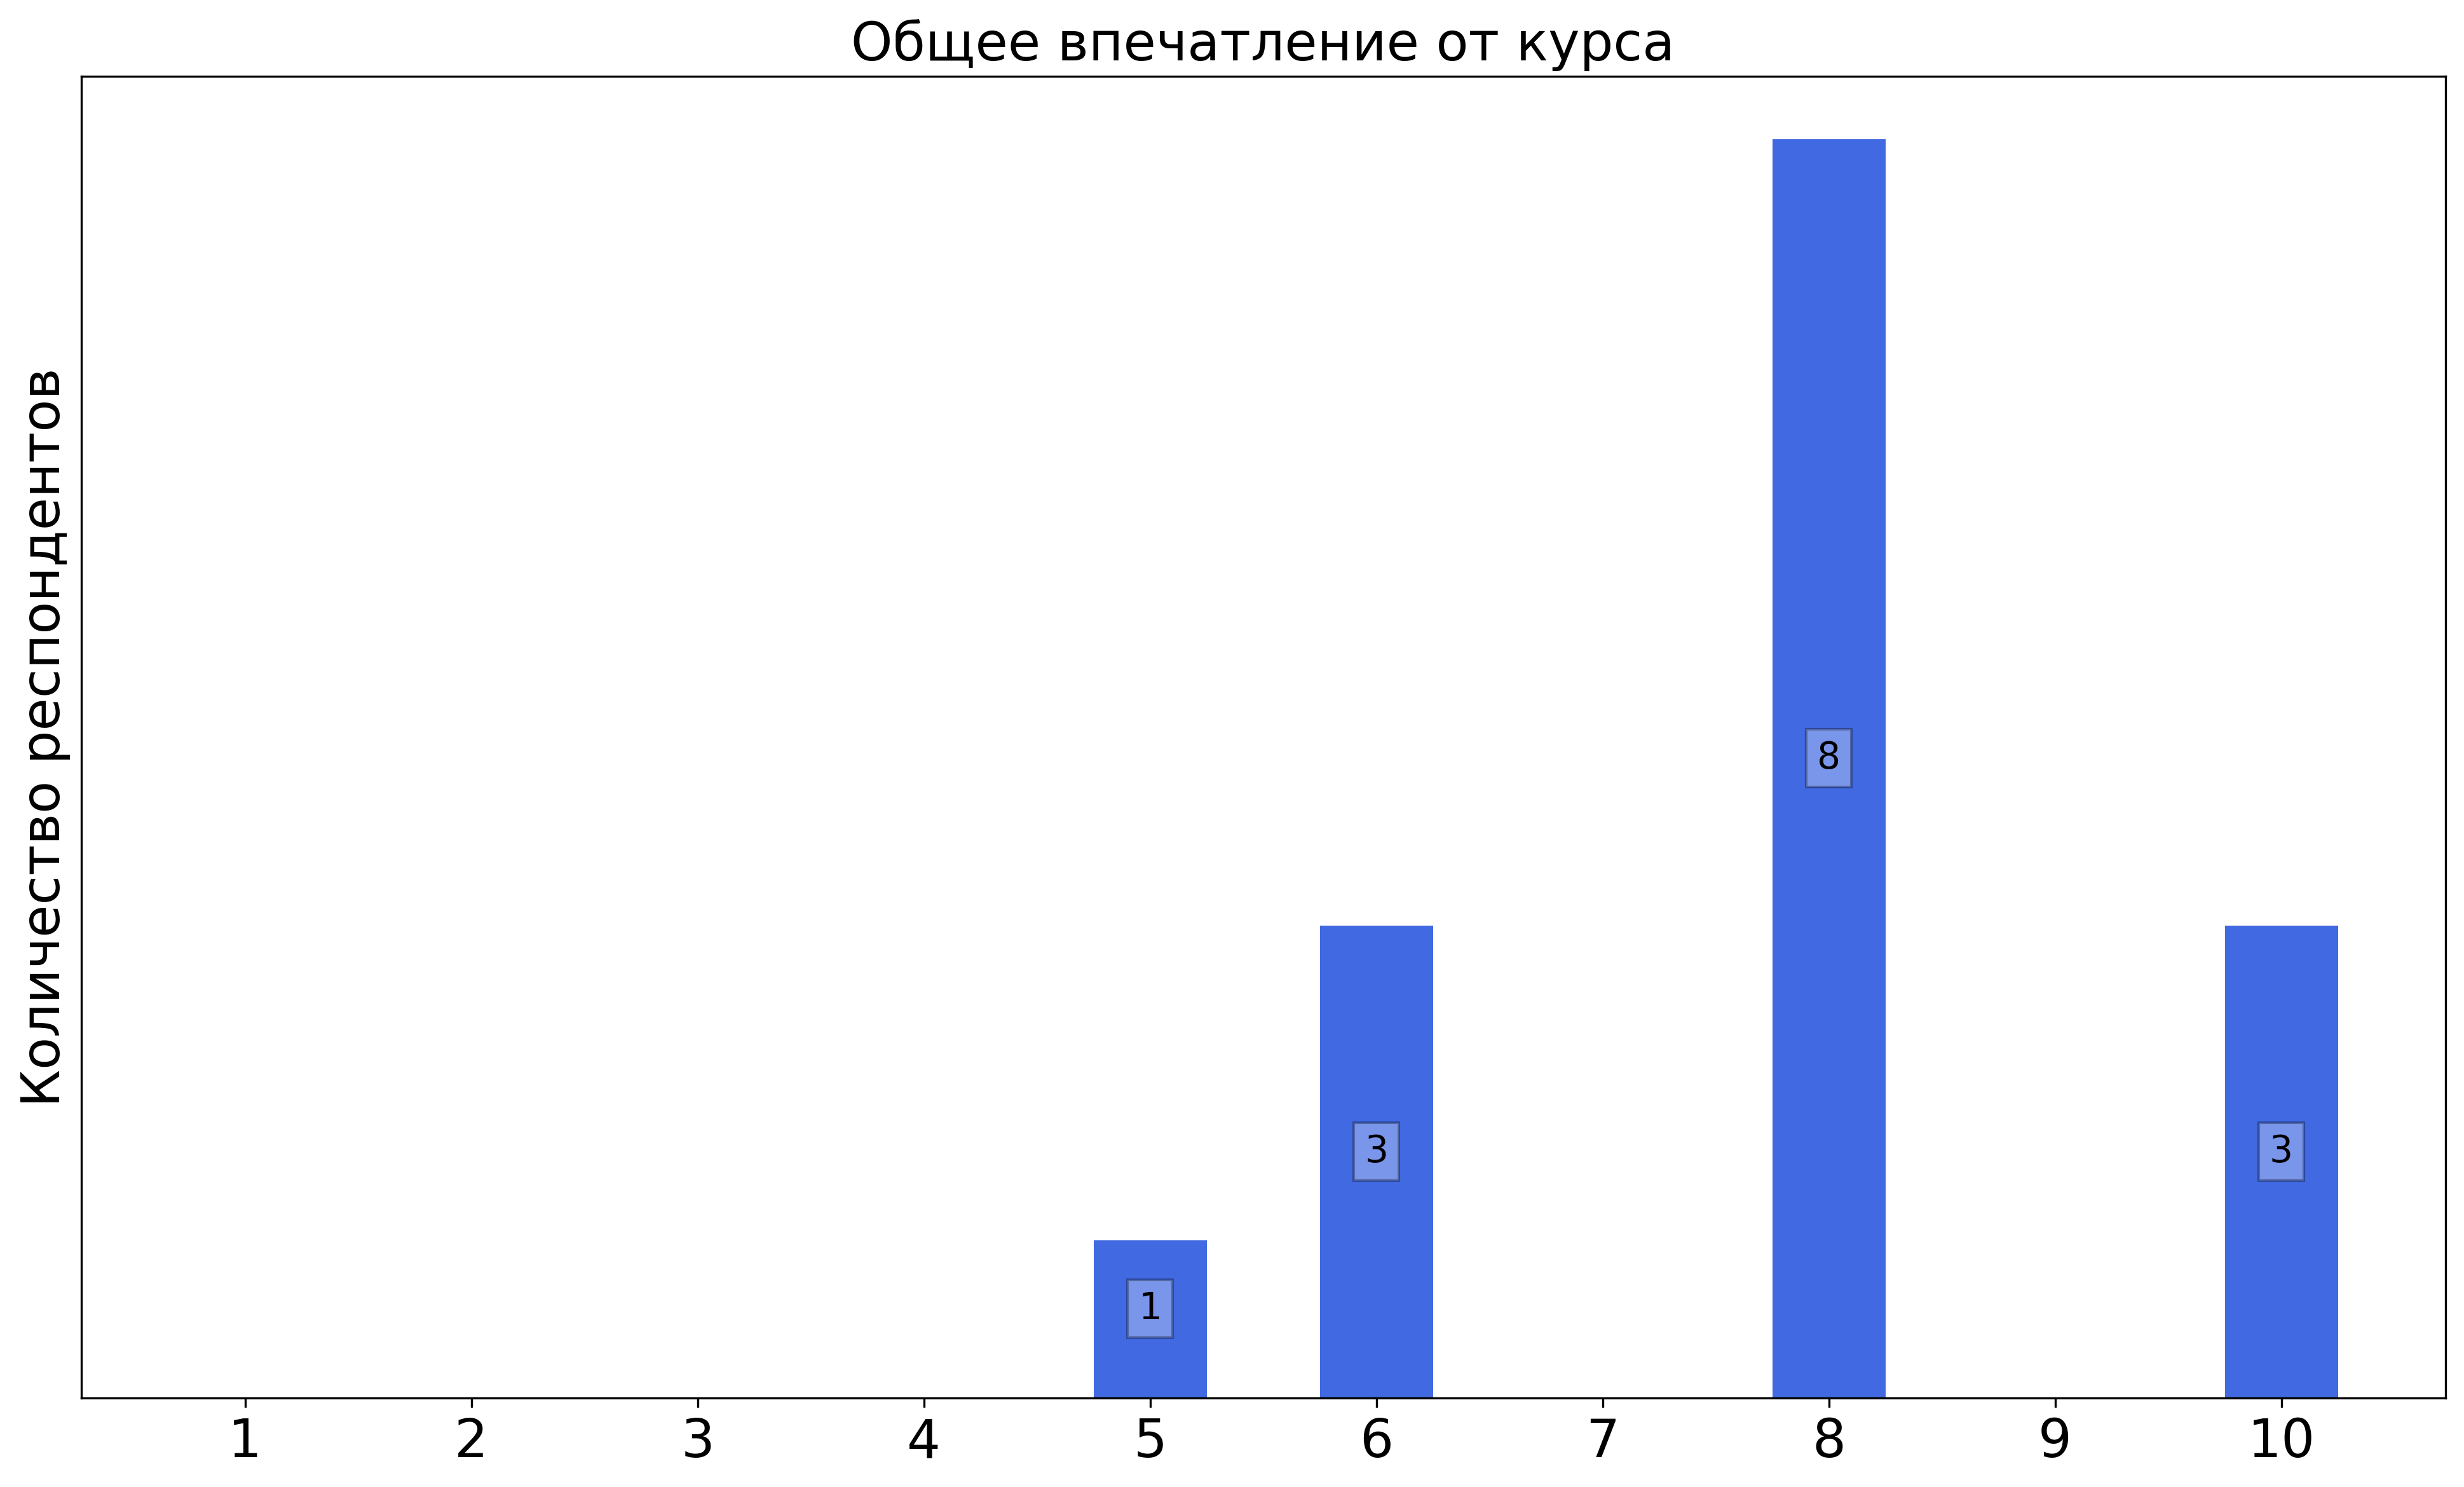
\includegraphics[width=\textwidth]{images/4 course/Теория информации/general-0.png}
			\end{subfigure}
		\end{figure}

	\subsubsection{Материалы, использумые респондентами при изучении курса}

		\begin{figure}[H]
			\centering
			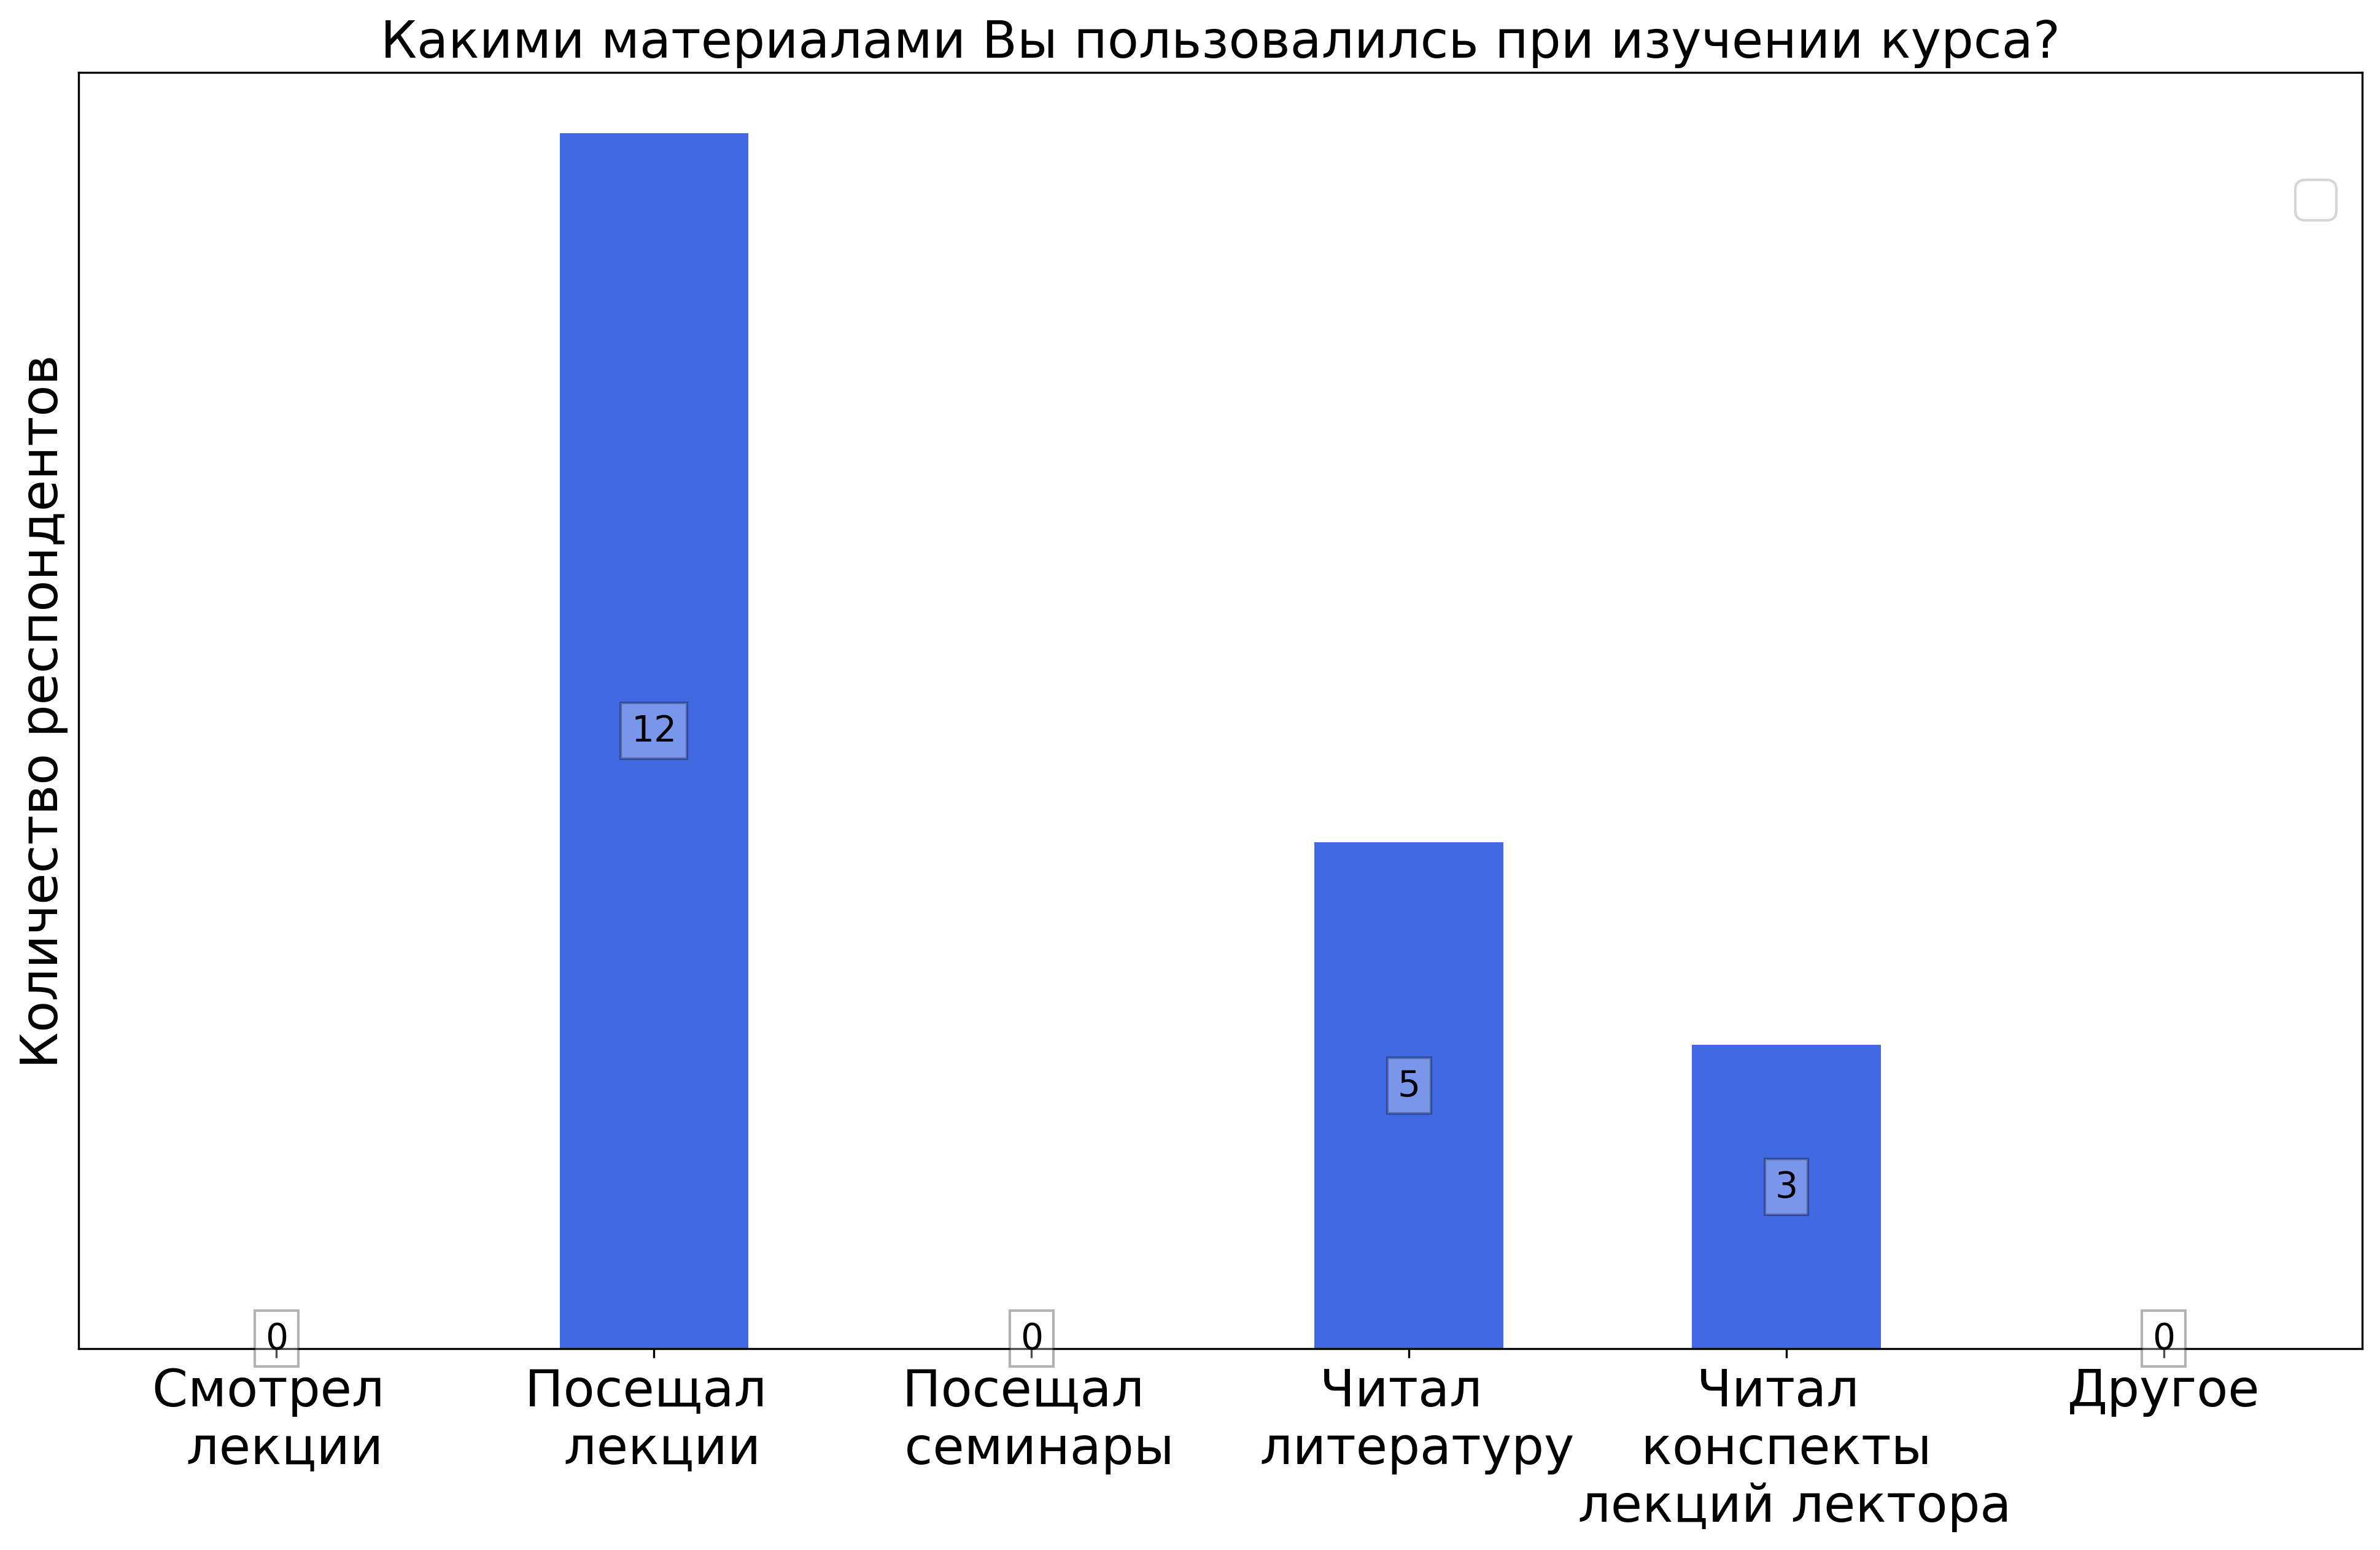
\includegraphics[width = 0.45\textwidth]{images/4 course/Теория информации/materials.png}
		\end{figure}

	\subsubsection{Отзыв студентов о лекциях. Лектор: Григорьев А.А.}

		\begin{figure}[H]
			\centering
            \begin{subfigure}[b]{0.45\textwidth}
				\centering
				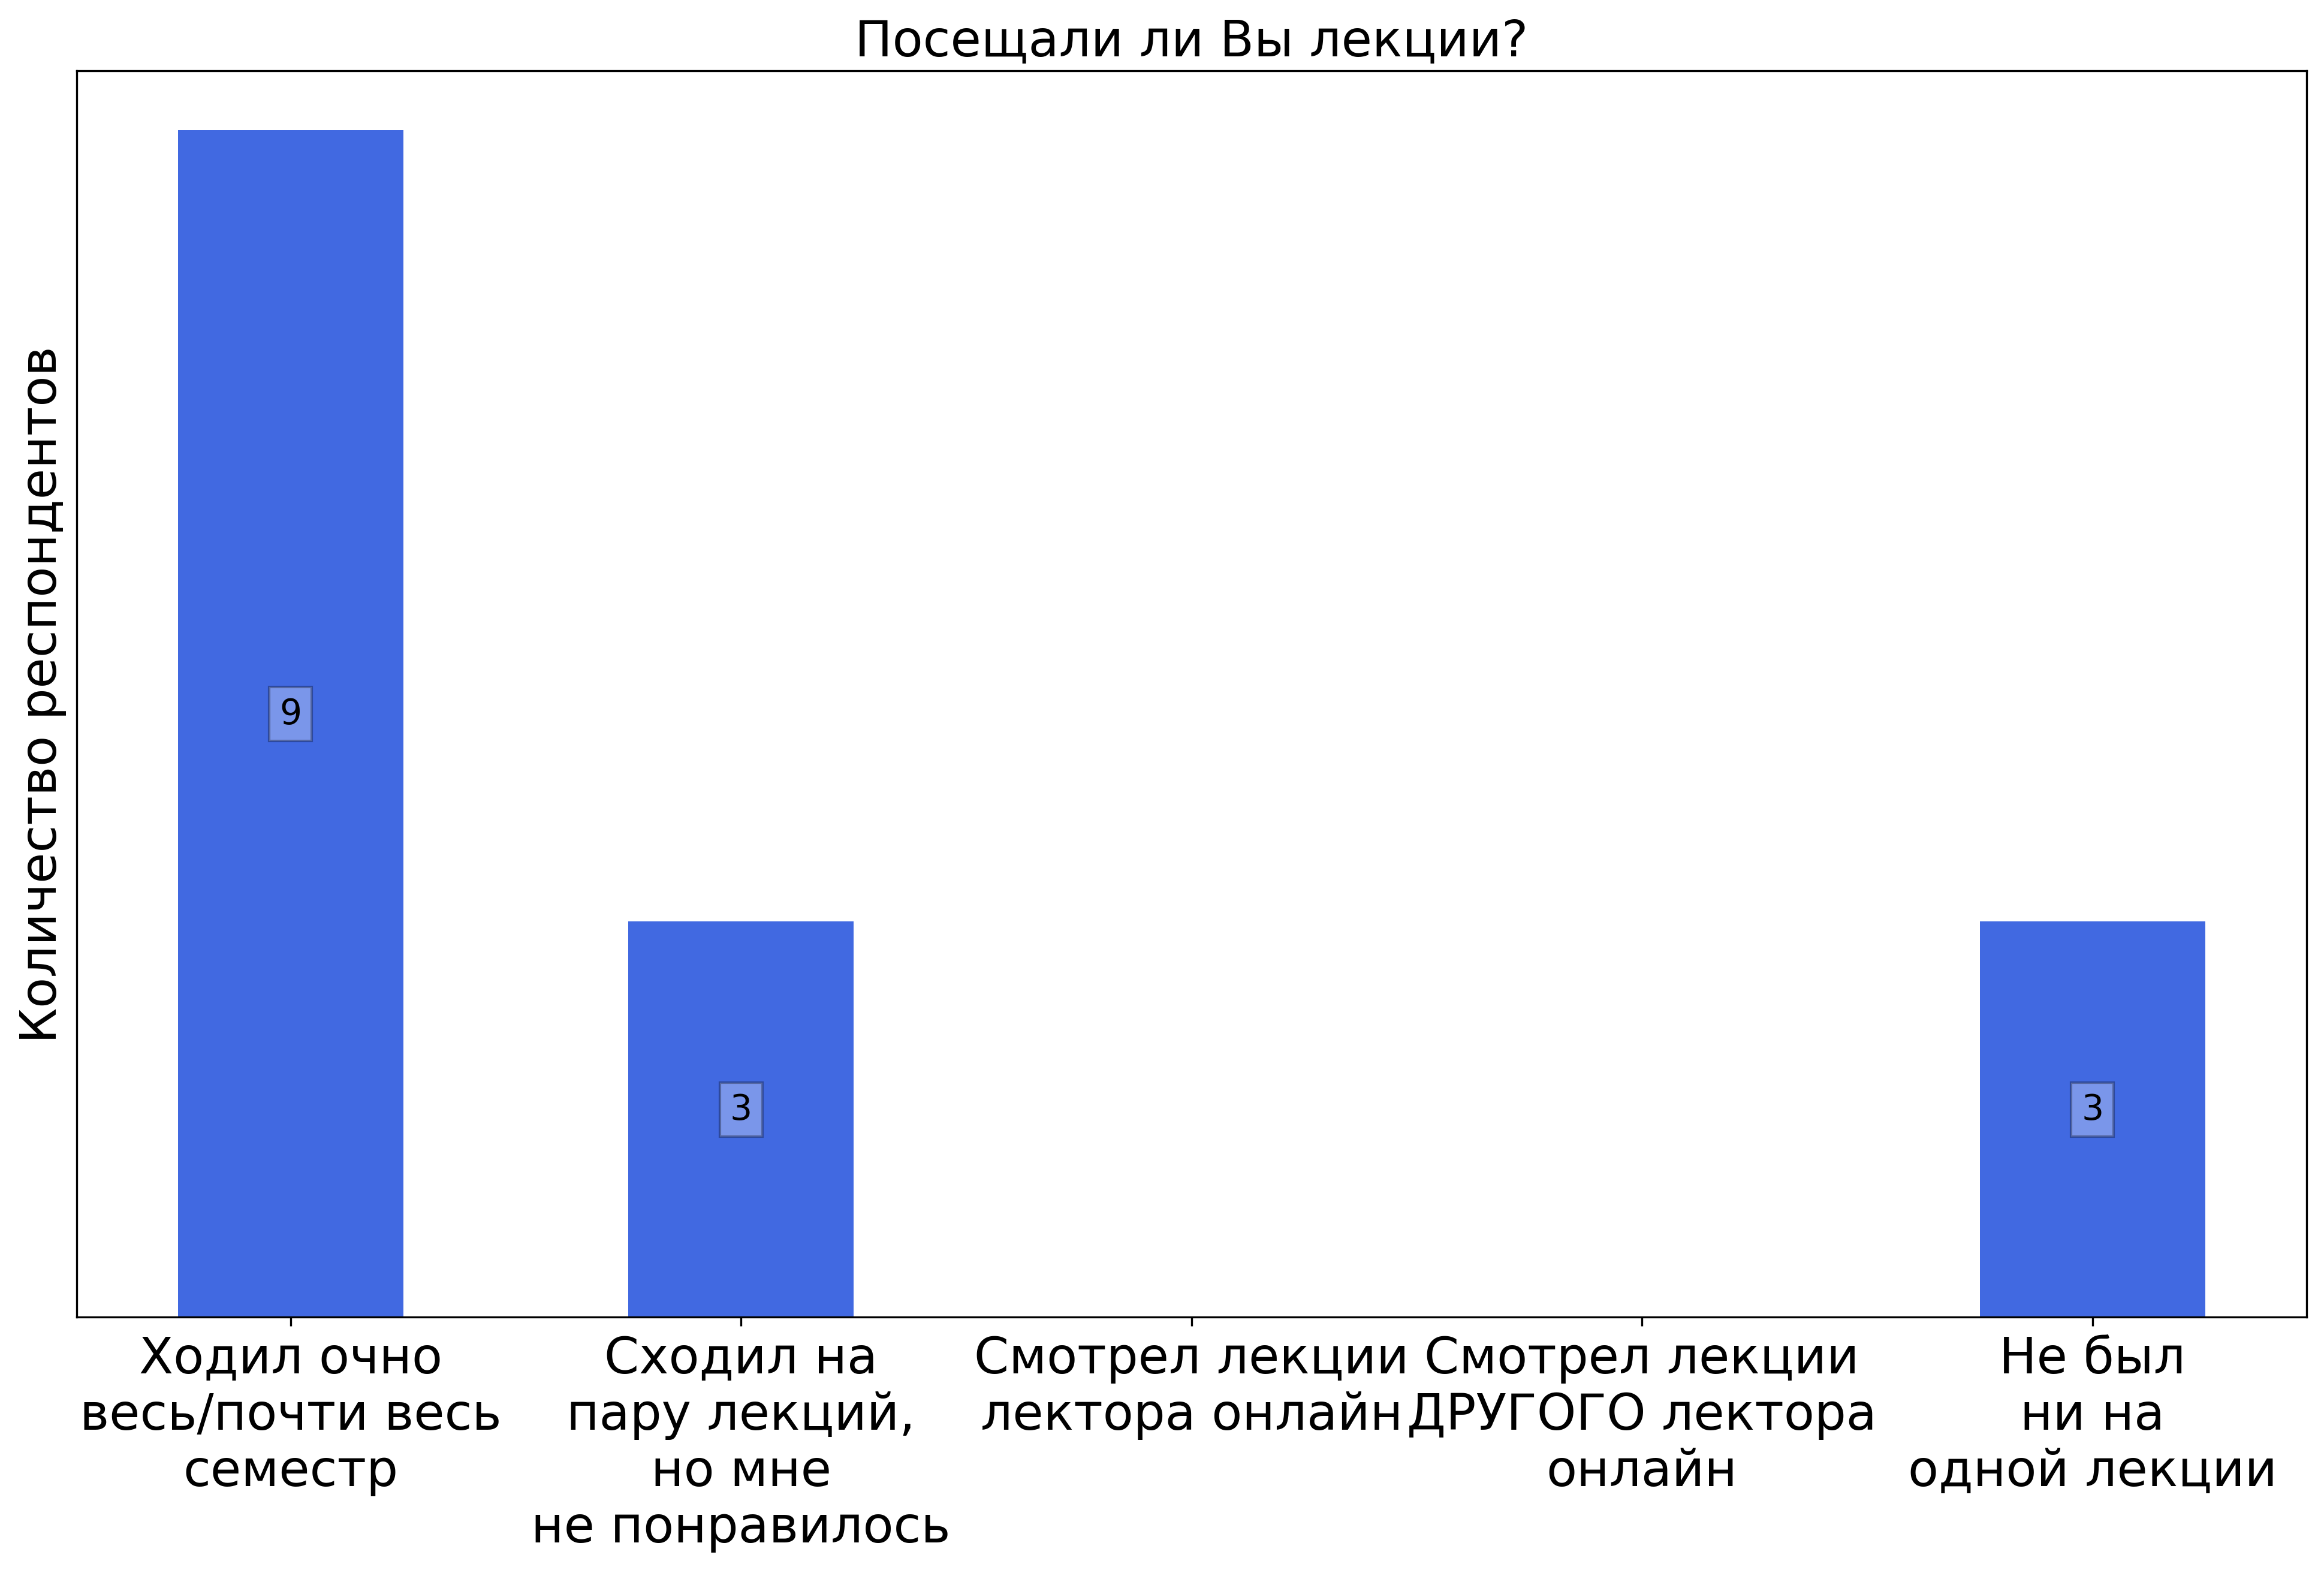
\includegraphics[width=\textwidth]{images/4 course/Теория информации/lecturer-questions-Григорьев А.А.-0.png}
			\end{subfigure}
			\begin{subfigure}[b]{0.45\textwidth}
				\centering
				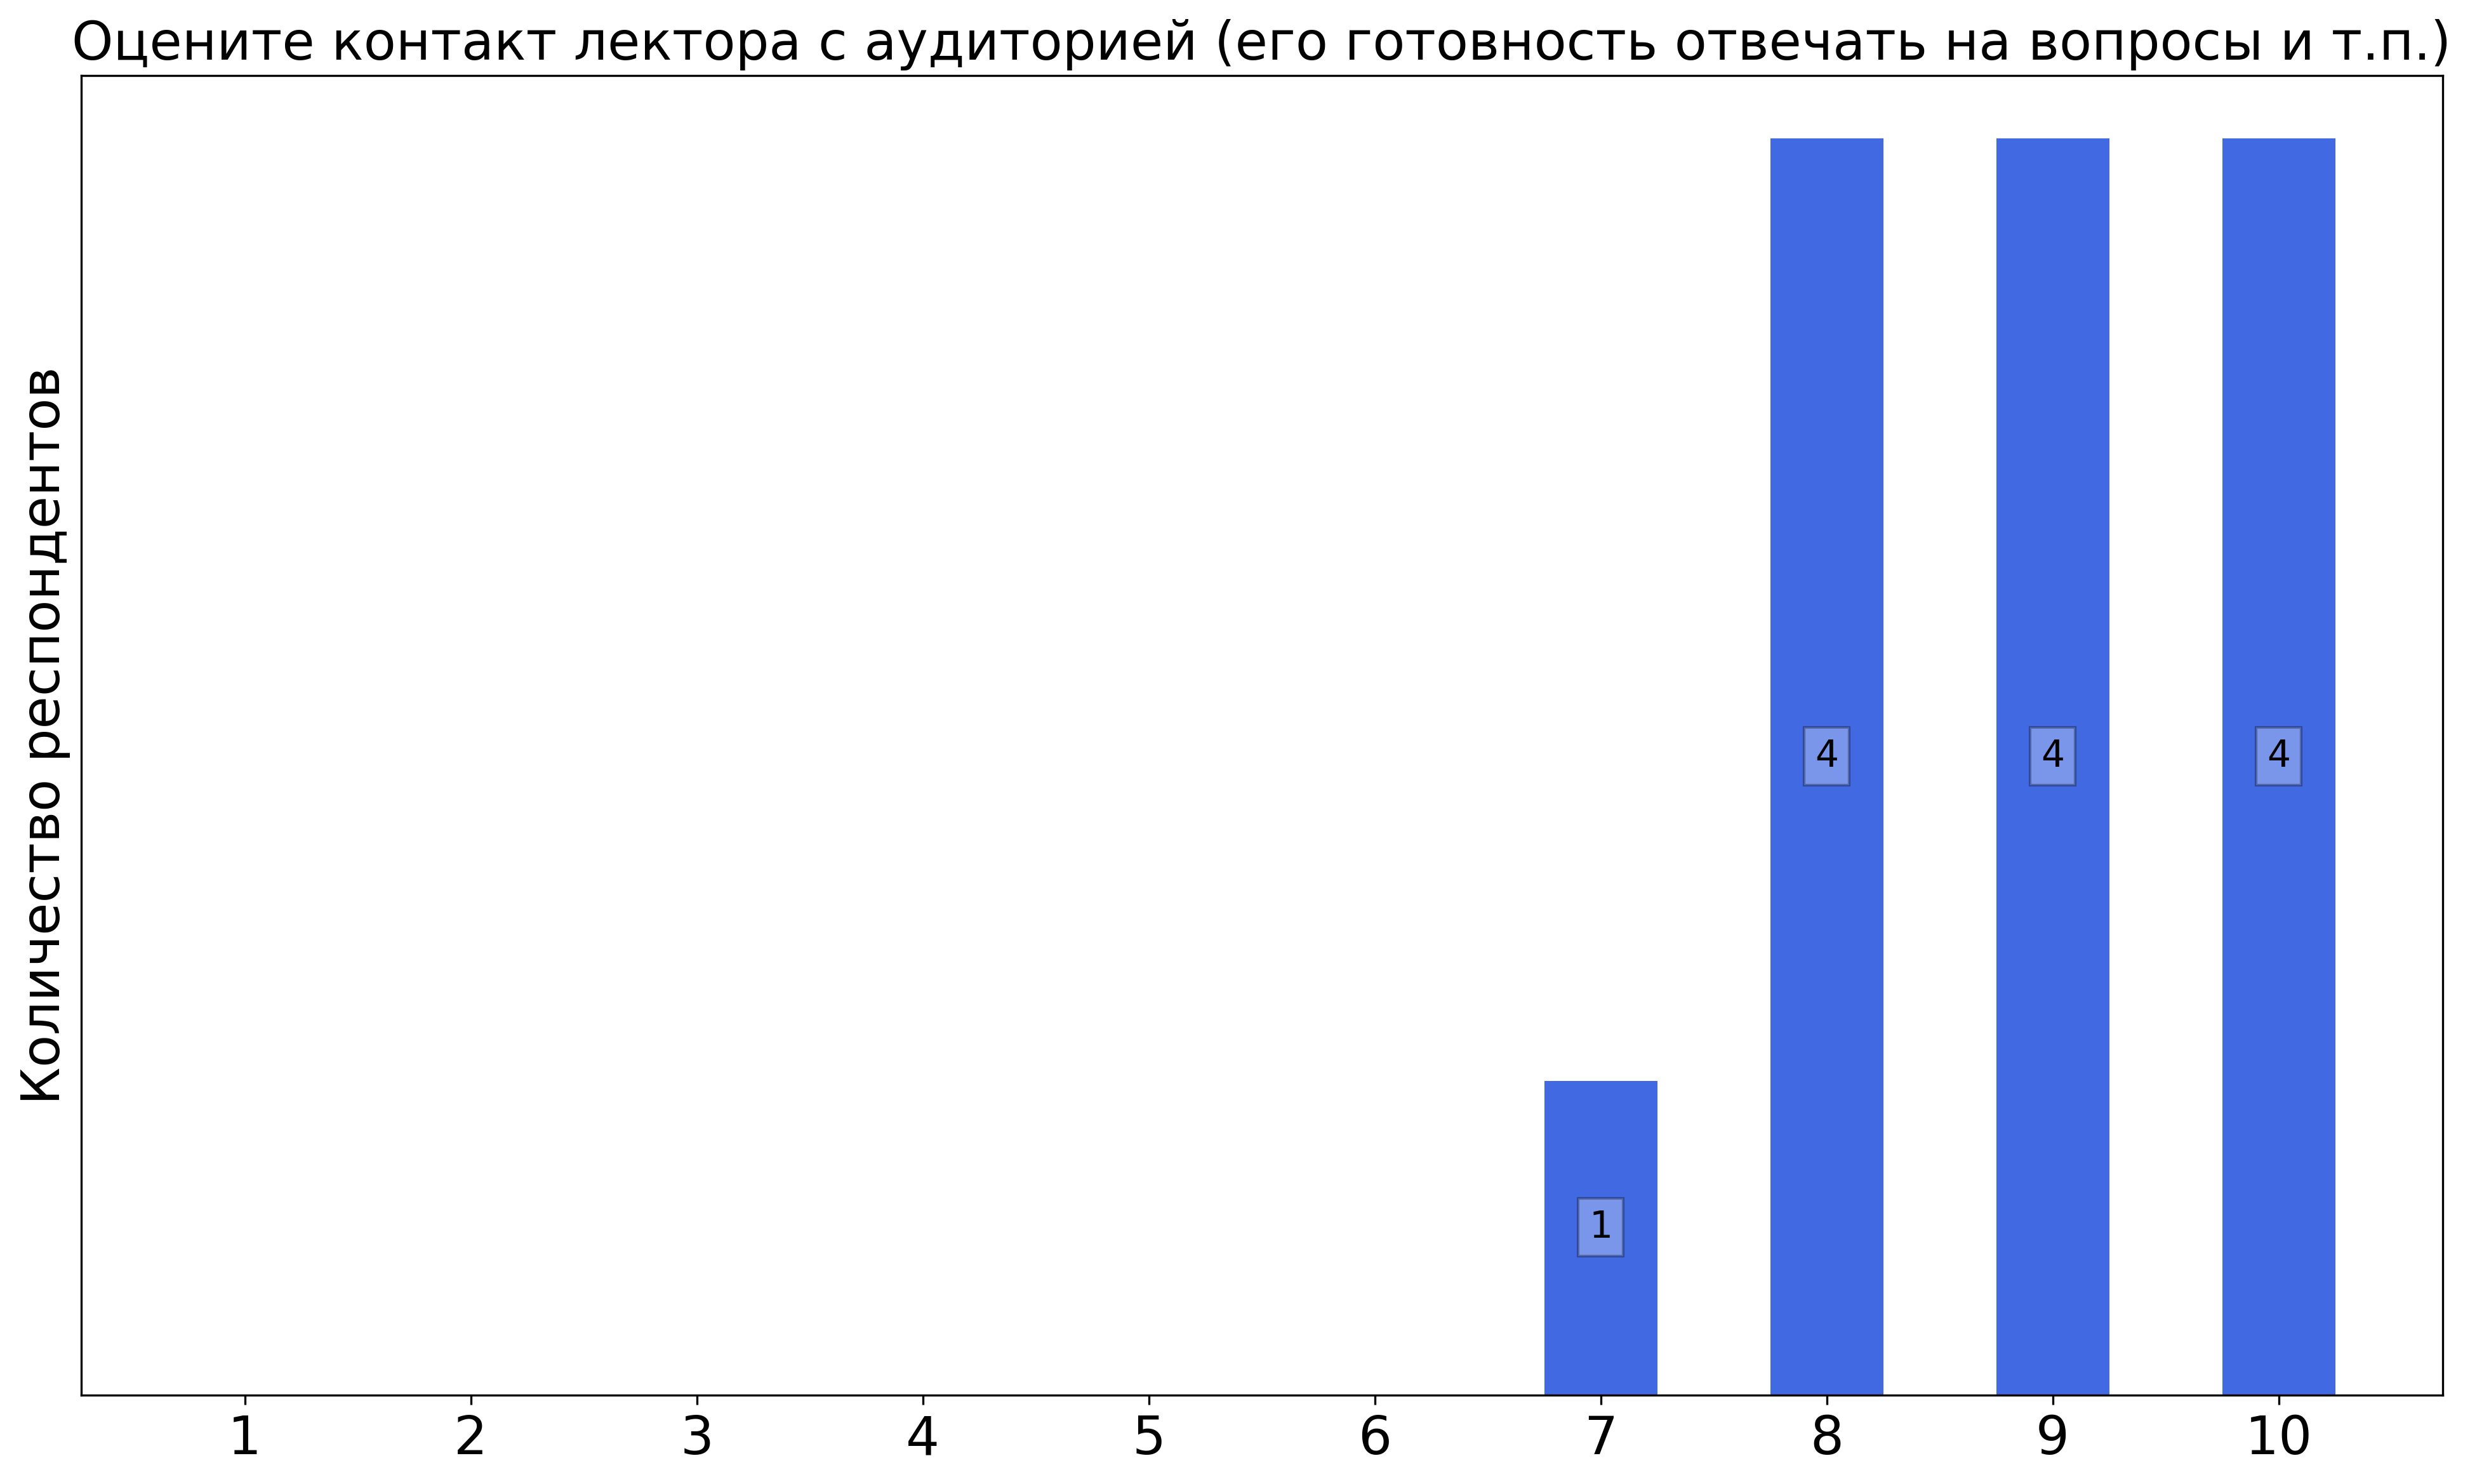
\includegraphics[width=\textwidth]{images/4 course/Теория информации/lecturer-marks-Григорьев А.А.-0.png}
			\end{subfigure}
			\begin{subfigure}[b]{0.45\textwidth}
				\centering
				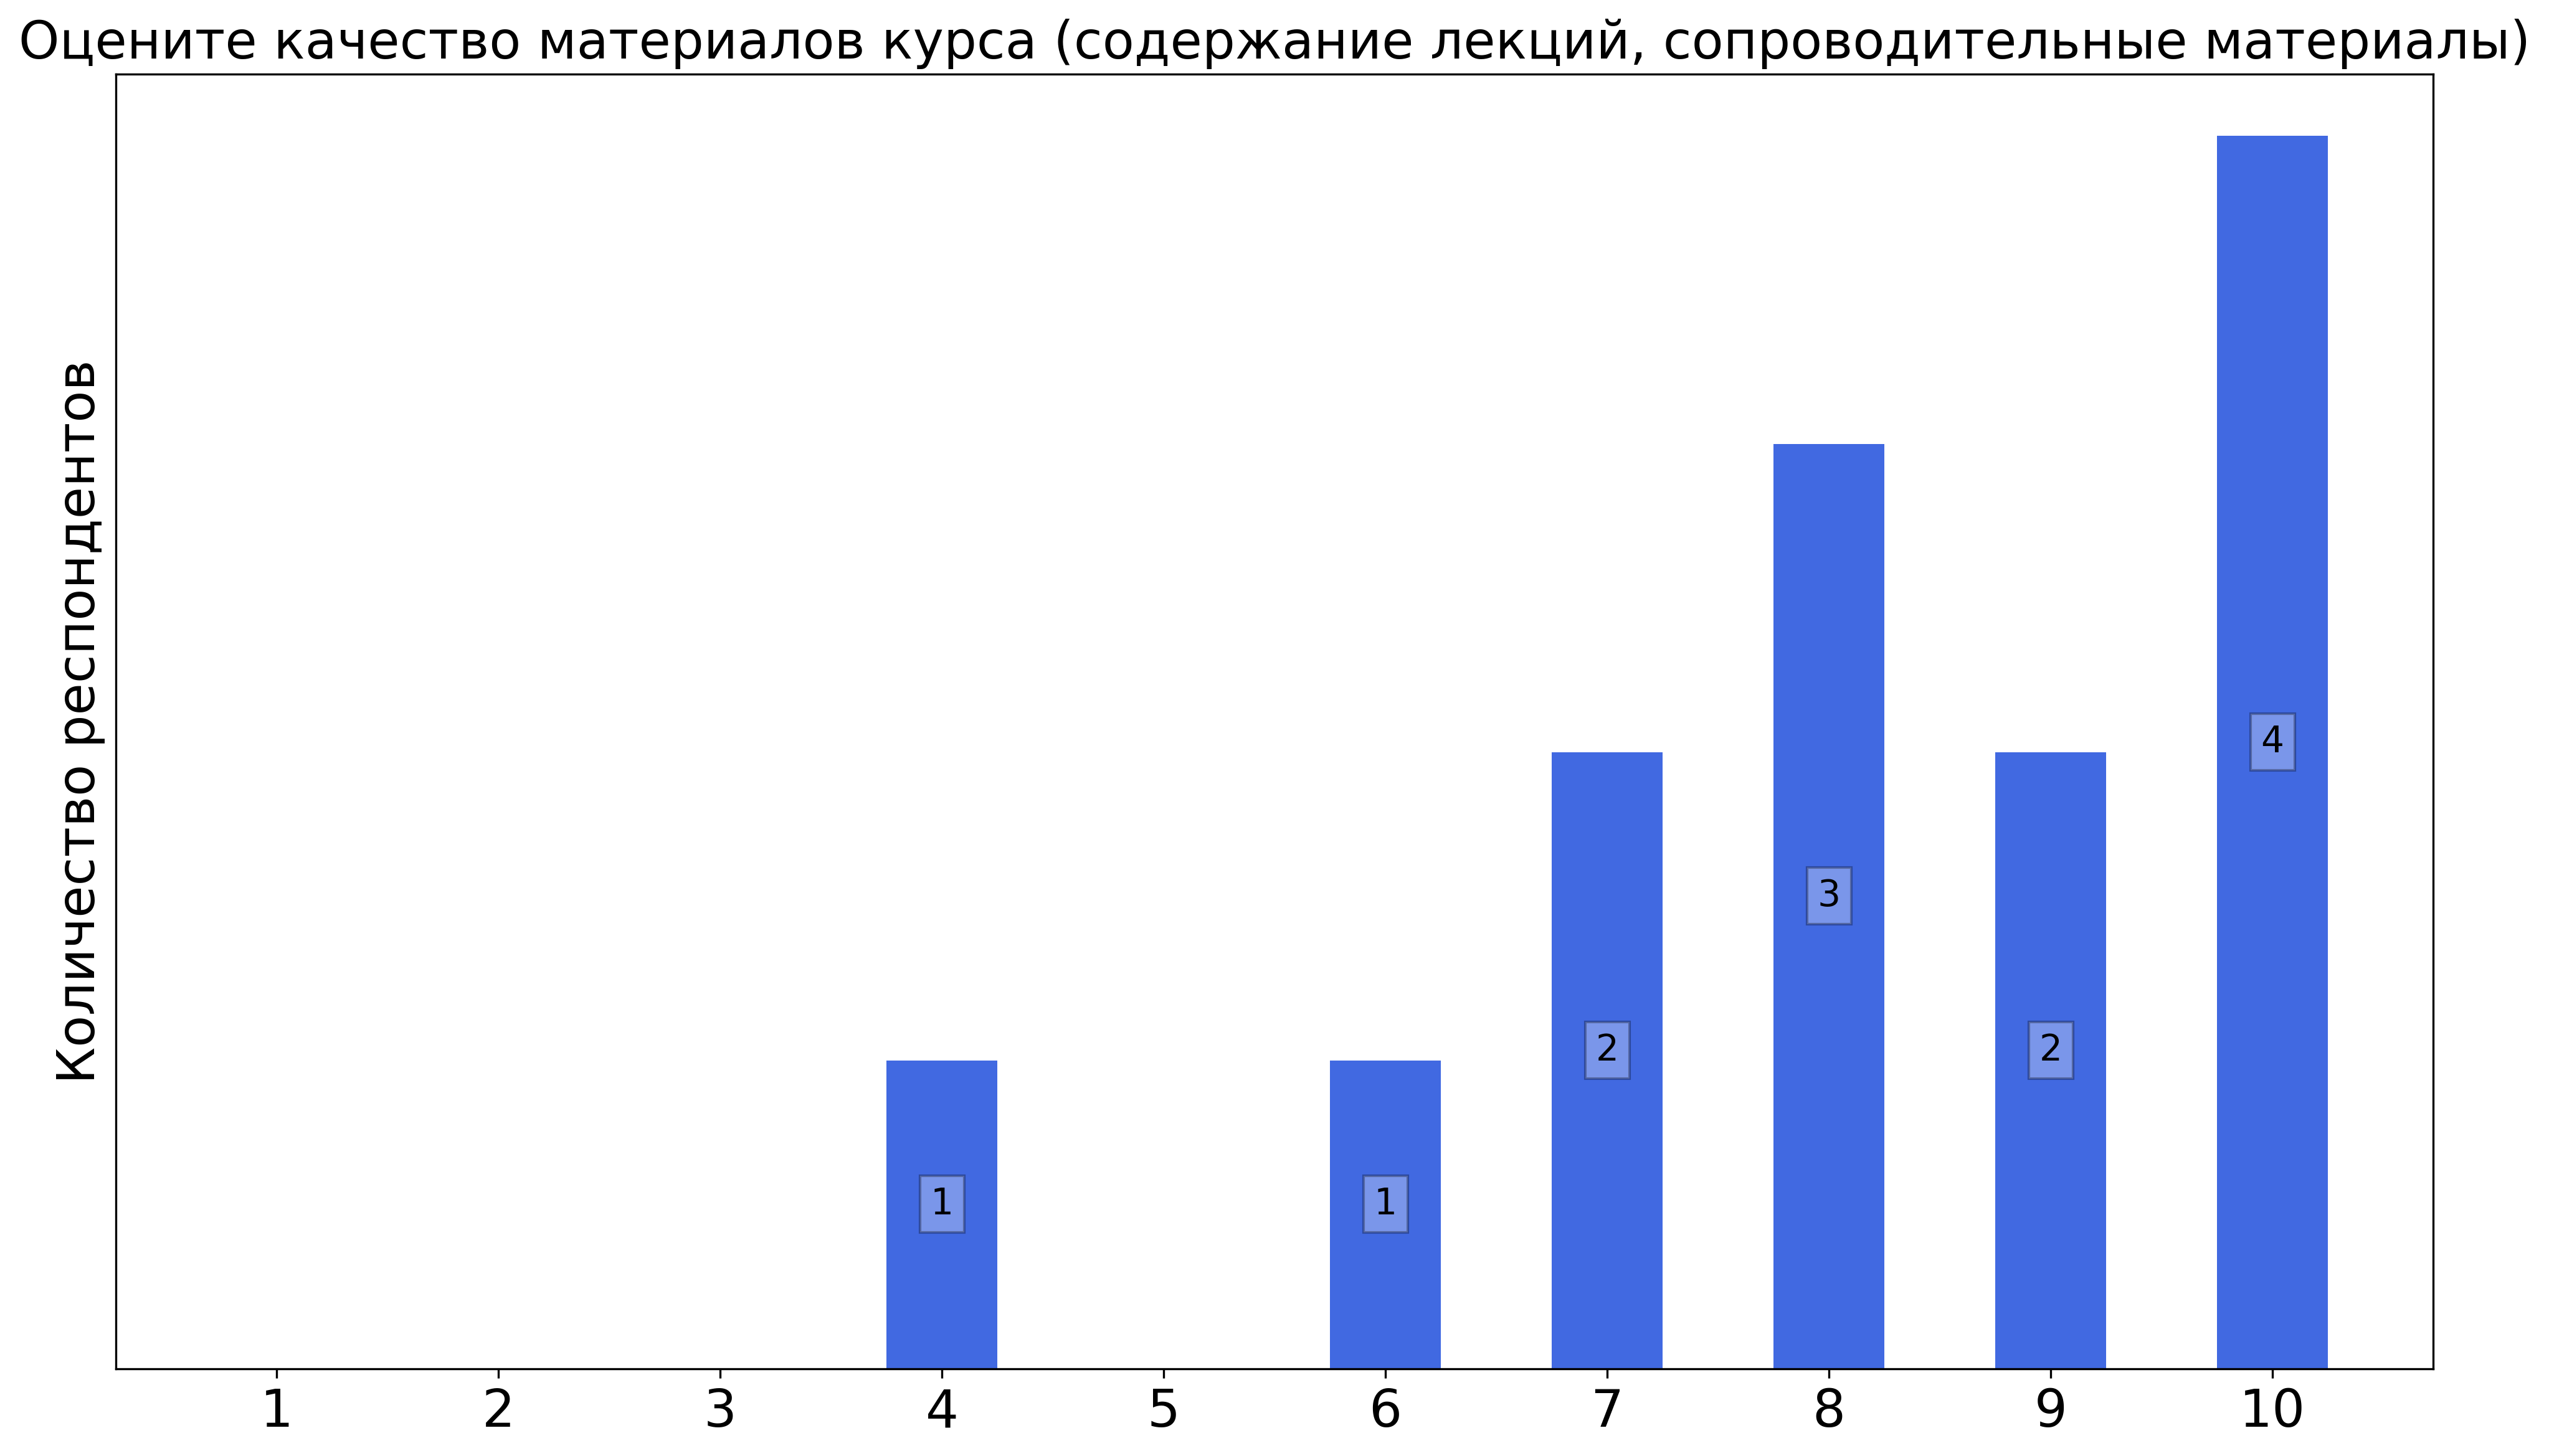
\includegraphics[width=\textwidth]{images/4 course/Теория информации/lecturer-marks-Григорьев А.А.-1.png}
			\end{subfigure}
			\begin{subfigure}[b]{0.45\textwidth}
				\centering
				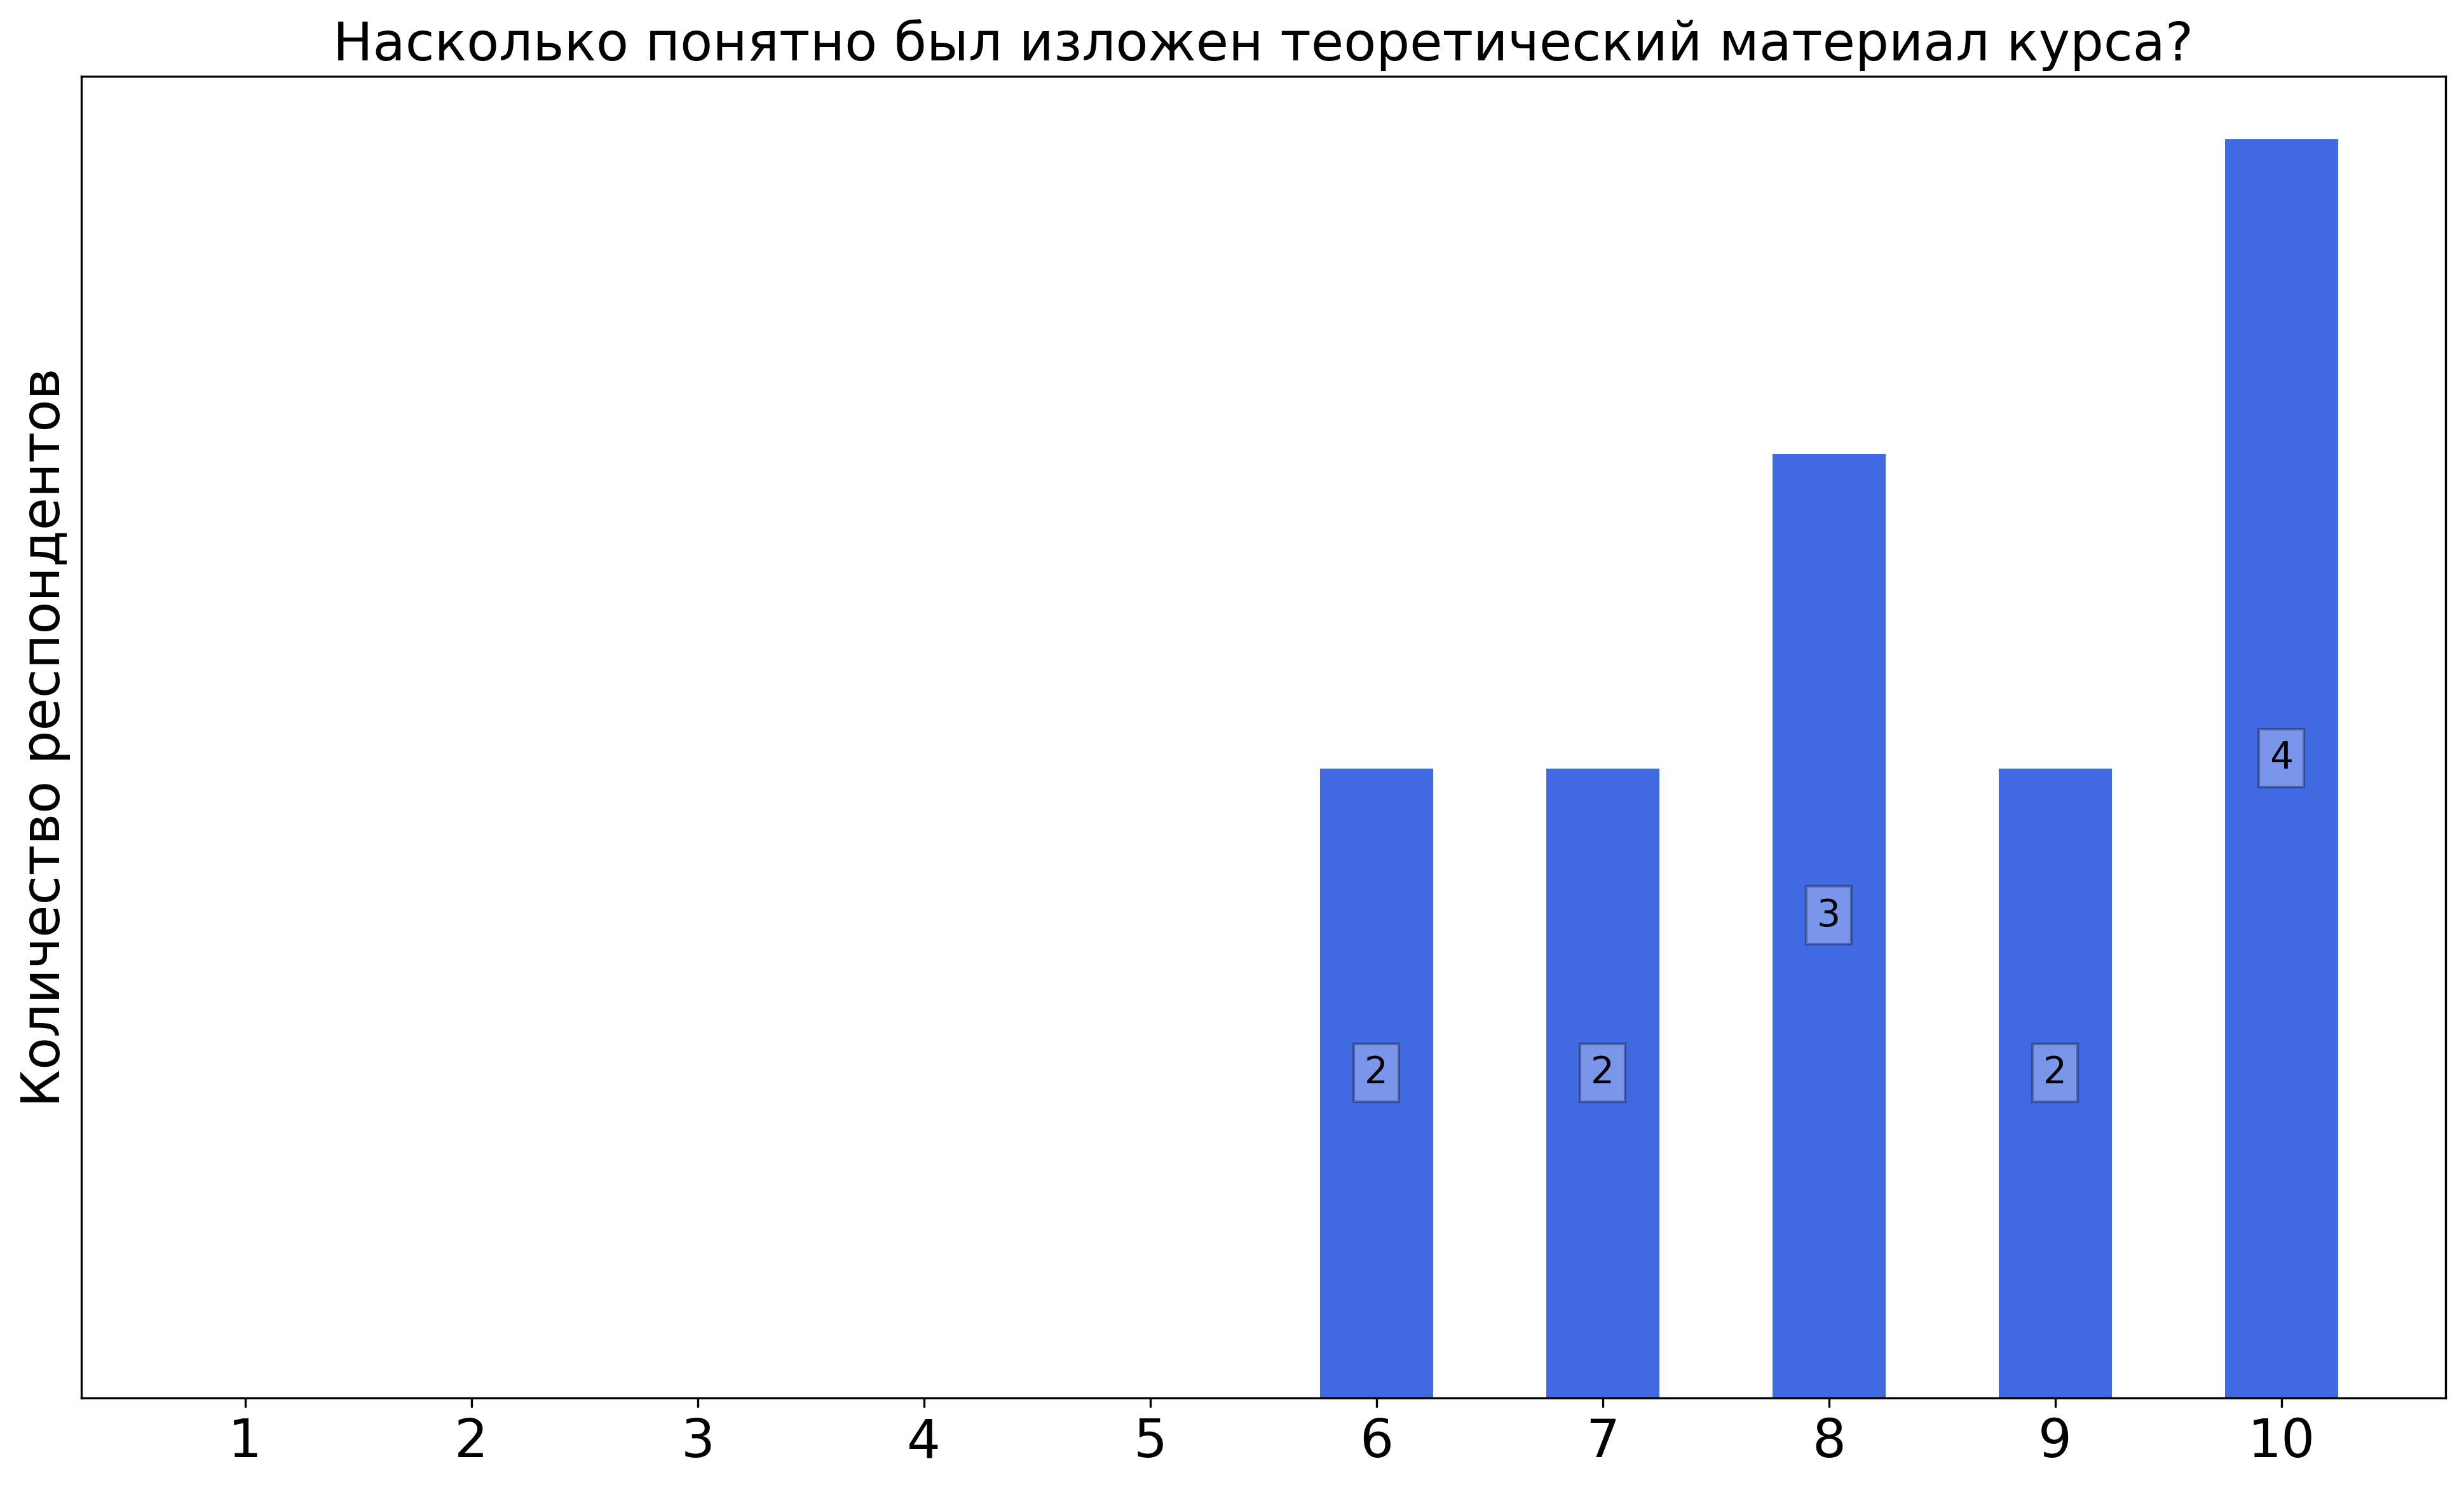
\includegraphics[width=\textwidth]{images/4 course/Теория информации/lecturer-marks-Григорьев А.А.-2.png}
			\end{subfigure}	
			\begin{subfigure}[b]{0.45\textwidth}
				\centering
				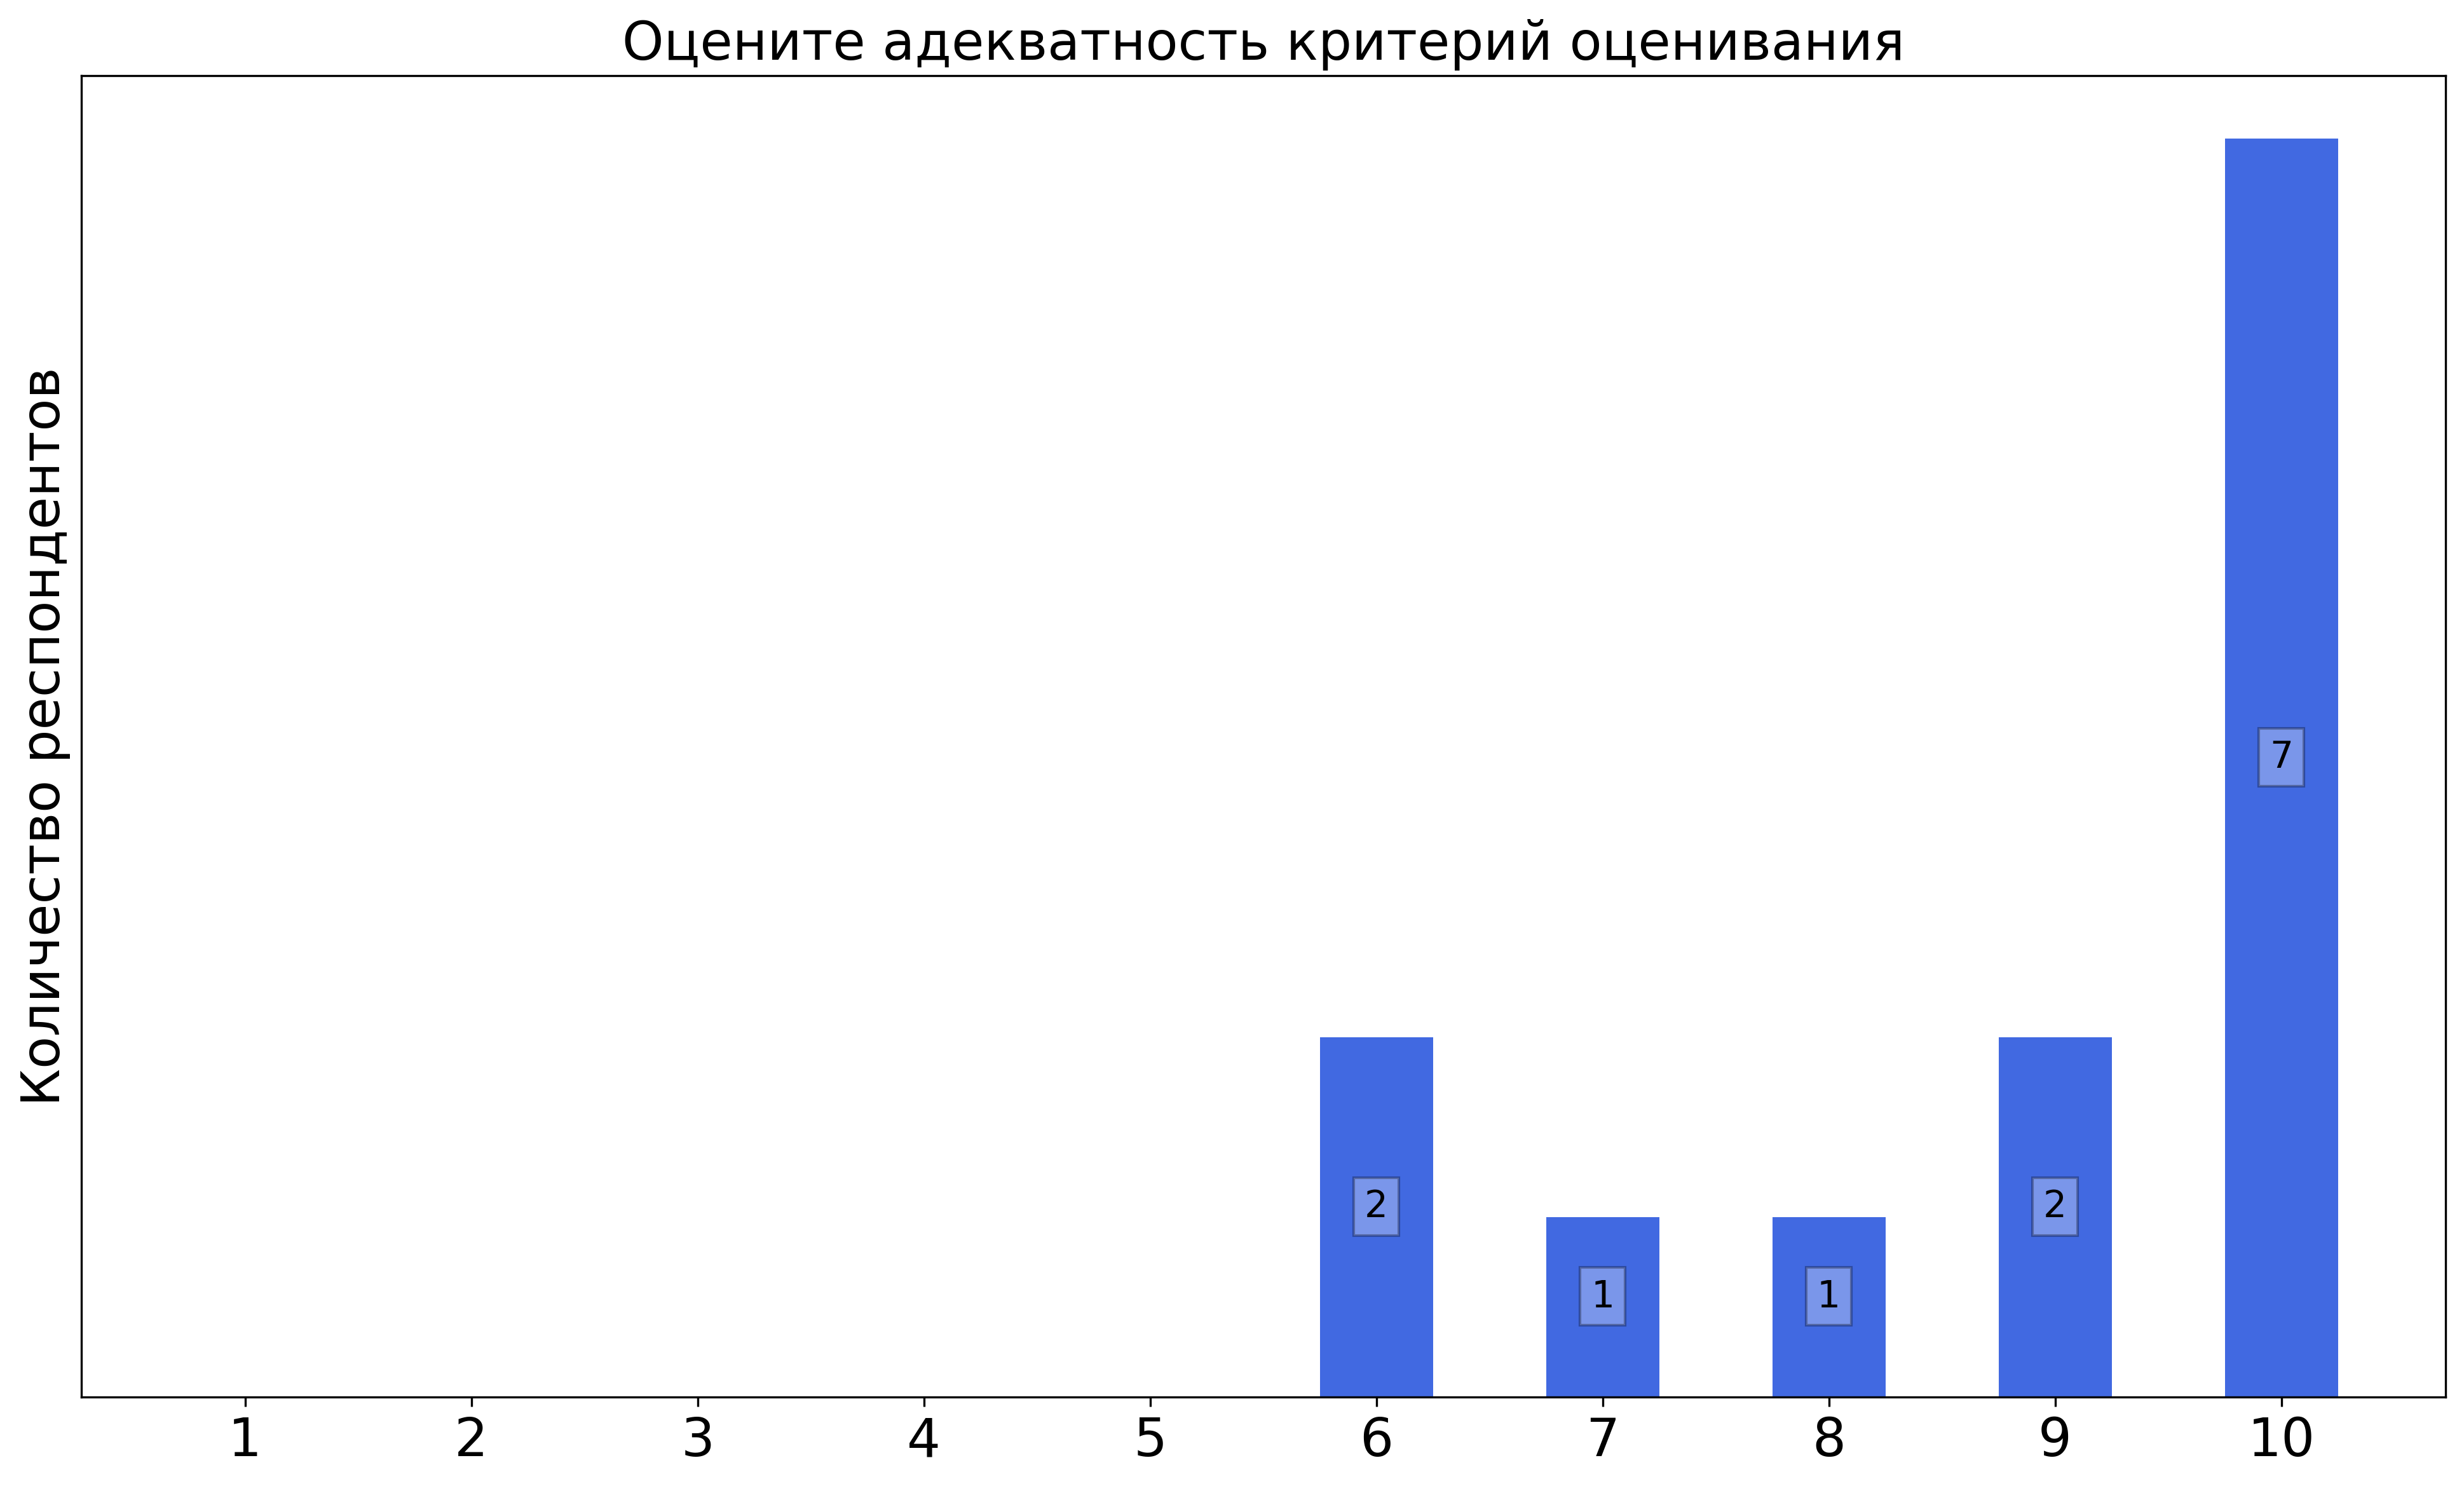
\includegraphics[width=\textwidth]{images/4 course/Теория информации/lecturer-marks-Григорьев А.А.-3.png}
			\end{subfigure}
			\caption{Оценки респондентов о качестве преподавания лекций по курсу <<Теория информации>>}
		\end{figure}

		\textbf{Комментарии студентов о лекциях\protect\footnote{сохранены оригинальные орфография и пунктуация}}
            \begin{commentbox} 
                Лектор живой и отвечает на вопросы. Однако лекции достаточно скучные. Слишком легко получить отличную оценку, по итогу курс ничему не учит...
            \end{commentbox} 
        
            \begin{commentbox} 
                Григорьев отлично рассказывает всегда, а еще не заставляет что то учить тех кто этого не хочет. Курс бывало немного пересекался с защитой информации и это мне понравилось. 
            \end{commentbox} 
        
            \begin{commentbox} 
                Ощущение, словно сейчас курс больше играет роль заглушки "что-то прочитали и слава Богу". Критерии  оценивания слишком халявные, семинаров нет, программа урезанная и слабая. Григорьев сам говорит что за 1 семестр он может только выбирать из огромного пласта материала хоть что-то что рассказать. Вот и выбрал понравившиеся темы. 
            \end{commentbox}     
    
    
    \subsubsection{Прочие комментарии и предложения по улучшению курса}
        \begin{commentbox}
            Полезнее было бы прослушать этот курс ранее, т.к. для понимания предмета достаточно знаний 1го-2го семестра. Так же необходимо вводить семинары по курсу, т.к. для глубинного понимания предмета необходимо увидеть, как знания с лекций используются на практике
        \end{commentbox}

        \begin{commentbox}
            Теория информации могла бы стоять раньше в учебном плане. Хотелось бы изучать ее более углублённо, чем сейчас предоставляет курс. 
        \end{commentbox}